\section{Checking for Saturated Subgraphs\label{sec:app1:saturated}}

This enhancement is based on the work in Ref.~\cite{Faulon2003b} for enumerating molecules. In their work, all atoms are mandatory in the graph. Therefore, the detection of a saturated subgraph before all atoms have been connected indicates the candidate graph will be infeasible and can be discarded.

\subsection{Theory}

A subgraph of a graph $G$ is another graph formed from a subset of the vertices and edges of $G$ \cite[p.~3]{Diestel2000a}.
A saturated subgraph is a subgraph with no empty ports and may contain multiple connected subgraphs \cite{Faulon2003b}.
Since a saturated subgraph has no empty ports, no components other than the components currently in this subgraph will be connected to this subgraph during further iterations of the graph generation procedure.
If we determine that the current iteration of the tree algorithm has created a saturated subgraph, then there are three scenarios to consider.

First, if all mandatory components are contained in the saturated subgraph, then no additional iterations are needed. Since all components not connected to a mandatory component will be removed, all components not currently in the saturated subgraph will be removed. Therefore, the topology of the remaining components is negligible. Since the topology is negligible, we can assign an arbitrary topology to the remaining components, save the graph, and terminate the iteration.

The second scenario is if none of the mandatory components are in the saturated subgraph. This provides no additional information so we allow the current iteration to continue. The final scenario is when some, but not all, mandatory components are in the saturated subgraph. Since at least one pair of mandatory components will not be connected, this graph will be infeasible. Therefore, we can terminate this iteration without saving the graph.

This is not a general enhancement since it requires specific NSCs, namely at least one mandatory component (\ref{ch2:s3}).

\subsection{Implementation}

\begin{vAlgorithm}[!ht]{1\columnwidth}{0em}
\LinesNumbered
\DontPrintSemicolon

\SetKw{Continue}{continue}

\SetKwFunction{find}{find}
\SetKwFunction{mysum}{sum}
\SetKwFunction{ismember}{ismember}
\SetKwFunction{any}{any}

\SetKwInOut{Input}{Input}
\SetKwInOut{Output}{Output}

\caption{Handle saturated subgraphs.\label{alg:app1:saturated}}

\Input{%
        \xvbox{2.5mm}{$\xvar{V}$} -- vector of remaining ports for each component replicate \\
        \xvbox{2.5mm}{$\xvar{E}$} -- vector of edges in sequential pairs \\
        \xvbox{2.5mm}{$\xvar{Vf}$} -- initial vector of ports available for each component replicate \\
        \xvbox{2.5mm}{$\xvar{M}$} -- vector indicating if all replicates of the component type must be present \\
        $\xvar{cVf}$ -- cumulative sum of the original $\xvar{V}$ plus 1 \\
        $\xvar{SavedGraphs}$ -- set of graphs \\
      }
\Output{%
        $\xvar{SavedGraphs}$ -- set of graphs
       }

\BlankLine

\If(){there are any necessary components}{
    
$\xvar{iNonSat}$ $\leftarrow$ $\find(\xvar{V})$ \tcc*{find the nonsaturated components}

\If(\tcc*[f]{check for saturated subgraph\label{alg:app1:saturated-l3}}){$\xvar{V}(\xvar{iNonSat}) = \xvar{Vf}(\xvar{iNonSat})$ }{

$\xvar{nUncon}$ $\leftarrow$ $\mysum(\xvar{M}(\xvar{iNonSat}))$ \tcc*{\# of mandatory comps not in saturated subgraph}

  \uIf(\tcc*[f]{all mandatory components are in saturated subgraph}){$\xvar{nUncon} = 0$}{

  \For(\tcc*[f]{add remaining edges in arbitrary order\label{alg:app1:saturated-l6}}){ $j$ $\leftarrow$ $1$ \KwTo $\mysum(\xvar{V})$}{

  {$k$} $\leftarrow$ $\find(\xvar{V},1)$ \tcc*{find first nonzero entry}

  {$\xvar{LR}$} $\leftarrow$ $\xvar{cVf}(k)-\xvar{V}(k)$ % \tcc*{port}

  {$\xvar{V}(k)$} $\leftarrow$ $\xvar{V}(k)-1$ \tcc*{remove port}

  {$\xvar{E}$} $\leftarrow$ $[\xvar{E},\xvar{LR}]$ \tcc*{add port}

  }

  $\xvar{SavedGraphs}\{\xvar{end}+1\}$ $\leftarrow$ $\xvar{E}$ \tcc*{missorted perfect matching}

  \Continue \tcc*{stop iteration, graph has been added \label{alg:app1:saturated-l13}}

}

\uElseIf(\tcc*[f]{no mandatory comps are in saturated subgraph\label{alg:app1:saturated-l14}}){$\xvar{nUncon} = \mysum(\xvar{M})$}{

  \tcc{continue with this iteration}

}

\Else(\tcc*[f]{some but not all mandatory components are in saturated subgraph\label{alg:app1:saturated-l15}}){

  \Continue  \tcc*{stop iteration, this graph is infeasible\label{alg:app1:saturated-l16}}

}

}

}

\end{vAlgorithm}

Algorithm~\ref{alg:app1:saturated} is the pseudocode for the implementation of this enhancement.
This enhancement is only called if there are some mandatory components ($S_3$).
First, the unsaturated components are found by checking the vector of remaining ports for each component replicate, $\xvar{V}$. A component is saturated if all ports are filled.
To determine if the current graph is a saturated subgraph, we compare the remaining ports of the unsaturated components to the original number of ports available (see line~\ref{alg:app1:saturated-l3}).

If the current graph is indeed a saturated subgraph, then we compute the number of mandatory components not in the saturated subgraph, $\xvar{nUncon}$.
If all mandatory components are in the saturated subgraph, then this graph is feasible. We assign an arbitrary ordering to the remaining components, save the graph, and terminate the iteration (see lines~\ref{alg:app1:saturated-l6} to \ref{alg:app1:saturated-l13}).
If no mandatory components are in the saturated subgraph, then we allow the current iteration to continue (see line~\ref{alg:app1:saturated-l14}).
Finally, if some but not all mandatory components are in the saturated subgraph, we stop the iteration since the graph is infeasible (see lines~\ref{alg:app1:saturated-l15} and \ref{alg:app1:saturated-l16}).

This enhancement is inserted between lines~\ref{alg:app1:tree-A2} and \ref{alg:app1:tree-if} of Alg.~\ref{alg:app1:tree} since the current edge needs to be added but before the recursion call.
With this enhancement, the \texttt{else} statement on line~\ref{alg:app1:tree-else} of Alg.~\ref{alg:app1:tree} will never be reached if there are any mandatory components.
The \texttt{if} condition is only untrue when a saturated subgraph is present (every component's port being filled).

\subsection{Examples}

\subsubsection{Example 1\label{sec:app1:saturated-ex1}}

The base three-tuple and NSCs for this example are specified as:
\begin{align}
C = \{ \xcolor{X}, \xcolor{Y} \}, \quad R = [2\ 3], \quad P = [2\ 2], \quad S_3 \text{ with } M = [1\ 0]
\end{align}

\noindent Some of the other inputs are then:
\begin{align}
\xvar{Vf} = [2\ 2\ 2\ 2\ 2], \quad \xvar{M} = [1\ 1\ 0\ 0\ 0]
\end{align}

\noindent We will consider two different $\xvar{V}$, one after an initial edge is added and one at some intermediate iteration. Figure~\ref{tb:app1:saturated-ex1-V} goes through the operations in Algorithm~\ref{alg:app1:saturated} for the different $\xvar{V}$.
These example iterations are also visualized in Figs.~\ref{fig:app1:saturated-ex1-original} and \ref{fig:app1:saturated-ex1-intermediate}.

Table~\ref{tb:app1:saturated-ex1} compares the original algorithm with the enhancement for this example. There is a reduction in candidate graphs generated while the number of unique graphs remains the same.

\begin{figure}[!ht]

\begin{subfigure}[b]{\textwidth}
\centering
\begin{tabular}{r | c | c}
 Iteration & Initial & Intermediate \\
 \hline 
 $\xvar{V}$ & [1 1 2 2 2] & [0 0 2 0 2] \\
 $\xvar{iNonSat}$ $\leftarrow$ $\find(\xvar{V})$ & [1 2 3 4 5] & [3 5] \\
 $\xvar{V}(\xvar{iNonSat})$ & [1 1 2 2 2] & [2 2] \\
 $\xvar{Vf}(\xvar{iNonSat})$ & [2 2 2 2 2] & [2 2] \\
 $\xvar{V}(\xvar{iNonSat}) = \xvar{Vf}(\xvar{iNonSat})$ & False & True \\
 $\xvar{M}(\xvar{iNonSat})$ & $-$ & [0 0] \\
 $\xvar{nUncon}$ $\leftarrow$ $\mysum(\xvar{M}(\xvar{iNonSat}))$ & $-$ & 0 \\
 Feasible & $-$ & Yes
\end{tabular}
\caption{Algorithm operations.\label{tb:app1:saturated-ex1-V}}
\end{subfigure}%

\begin{subfigure}[b]{0.5\textwidth}
\centering
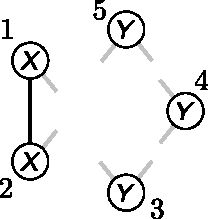
\includegraphics[scale=1]{../app1/fig/saturated-ex1-original_v2}
\caption{Initial iteration.\label{fig:app1:saturated-ex1-original}}
\end{subfigure}%
\begin{subfigure}[b]{0.5\textwidth}
\centering
 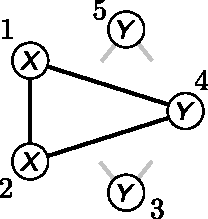
\includegraphics[scale=1]{../app1/fig/saturated-ex1-intermediate_v2}
 \caption{Intermediate iteration.\label{fig:app1:saturated-ex1-intermediate}}
\end{subfigure}%

\caption{\nameref{sec:app1:saturated-ex1} for Algorithm~\ref{alg:app1:saturated} (saturated subgraphs).}
\end{figure}

\begin{table}[!ht]
\centering
\caption{Comparison (saturated subgraphs, \nameref{sec:app1:saturated-ex1}).\label{tb:app1:saturated-ex1}}
\begin{tabular}{r | c | c | c}
\hline \hline
& Orig & En & Orig/En \\
\hline
Candidate Graphs & 146 & 91 & 1.60 \\ 
Unique Graphs & 6 & 6 & 1 \\
Generation Time (s) & 0.0056  & 0.0046 & 1.22 \\
Total Time (s) & 0.023  & 0.015 & 1.53 \\
\hline \hline
\end{tabular}
\end{table}

\subsubsection{Example 2\label{sec:app1:saturated-ex2}}

The base three-tuple and NSCs for this example are specified as:
\begin{align}
C = \{ \xcolor{X} \}, \quad R = [9], \quad P = [2], \quad S_3 \text{ with } M = [1]
\end{align}

\noindent Some of the other inputs are then:
\begin{align}
\xvar{Vf} = [2\ 2\ 2\ 2\ 2\ 2\ 2\ 2\ 2], \quad \xvar{M} = [1\ 1\ 1\ 1\ 1\ 1\ 1\ 1\ 1]
\end{align}

\noindent We will consider two different $\xvar{V}$, one after an initial edge is added and one at some intermediate iteration. Figure~\ref{tb:app1:saturated-ex2-V} goes through the operations in Algorithm~\ref{alg:app1:saturated} for the different $\xvar{V}$. These example iterations are also visualized in Figs.~\ref{fig:app1:saturated-ex2-intermediate1} and \ref{fig:app1:saturated-ex2-intermediate2}.

Table~\ref{tb:app1:saturated-ex2} compares the original algorithm with the enhancement for this example. There is a reduction in candidate graphs generated while the number of unique graphs remains the same.

\begin{figure}[!ht]

\begin{subfigure}[b]{\textwidth}
\centering
\begin{tabular}{r | c | c}
\hline \hline
& Intermediate 1 & Intermediate 2 \\
\hline 
$\xvar{V}$ & [0 0 0 1 2 1 2 2 2] & [0 0 0 0 2 0 2 2 2] \\
$\xvar{iNonSat}$ $\leftarrow$ $\find(\xvar{V})$ & [4 5 6 7 8 9] & [5 7 8 9] \\
$\xvar{V}(\xvar{iNonSat})$ & [1 2 1 2 2 2] & [2 2 2 2] \\
$\xvar{Vf}(\xvar{iNonSat})$ & [2 2 2 2 2 2] & [2 2 2 2] \\
$\xvar{V}(\xvar{iNonSat}) = \xvar{Vf}(\xvar{iNonSat})$ & False & True  \\
$\xvar{M}(\xvar{iNonSat})$ & $-$ & [1 1 1 1] \\
$\xvar{nUncon}$ $\leftarrow$ $\mysum(\xvar{M}(\xvar{iNonSat}))$ & $-$ & 4 \\
Feasible & $-$ & No \\
\hline \hline
\end{tabular}
\caption{Algorithm operations.\label{tb:app1:saturated-ex2-V}}
\end{subfigure}%

\begin{subfigure}[b]{0.5\textwidth}
\centering
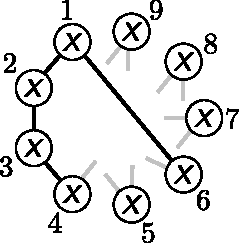
\includegraphics[scale=1]{../app1/fig/saturated-ex2-intermediate1_v2}
\caption{Intermediate 1 iteration.\label{fig:app1:saturated-ex2-intermediate1}}
\end{subfigure}%
\begin{subfigure}[b]{0.5\textwidth}
\centering
 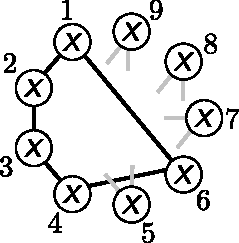
\includegraphics[scale=1]{../app1/fig/saturated-ex2-intermediate2_v2}
 \caption{Intermediate 2 iteration.\label{fig:app1:saturated-ex2-intermediate2}}
\end{subfigure}%

\caption{\nameref{sec:app1:saturated-ex2} for Algorithm~\ref{alg:app1:saturated} (saturated subgraphs).}
\end{figure}

\begin{table}[!ht]
\centering
\caption{Comparison (saturated subgraphs, \nameref{sec:app1:saturated-ex2}).\label{tb:app1:saturated-ex2}}
\begin{tabular}{r | c | c | c}
\hline \hline
& Orig & En & Orig/En \\
\hline
Candidate Graphs & 852316 & 460872 & 1.85 \\ 
Unique Graphs & 1 & 1 & 1 \\
Generation Time (s) & 29.83 & 19.23 & 1.55 \\
Total Time (s) & 58.57 & 33.11 & 1.77 \\
\hline \hline
\end{tabular}
\end{table}